\documentclass[12pt, a4paper]{article}

\usepackage{graphicx}
\graphicspath{ {./images/} }
%Tarih Ekleme
\usepackage[ddmmyyyy]{datetime}
\renewcommand{\dateseparator}{.}
\renewcommand{\figurename}{Şekil}
\renewcommand{\refname}{Kaynakça}




\title{Kıyafetleri Artırılmış Gerçeklik ile Gösterme}
\author{Hasan Tekin}
\date{\today}
%\date{\DTMnow}
%\date{\DTMnow}


\begin{document}
	\maketitle
    
    
    
    
	\section{Giriş}
	Günümüzde alışveriş, popüler bir aktivite olmanın yanı sıra zaman alan bir süreç halini almıştır. Kıyafet alışverişi, bazı insanlar için keyifli bir boş zaman etkinliği iken, diğerleri için ise uygun bir giysi seçimi yapabilmek adına yapılan tahmin çalışmalarının yoğunluğu nedeniyle stresli ve sıkıcı bir deneyim olabilir.
	
	Bu bağlamda, sanal giyinme odaları, alışveriş sürecini daha etkili ve keyifli hale getirebilen önemli bir teknolojik gelişmedir. Alışveriş yapanlara, fiziksel olarak giyinme odalarında deneme yapmak yerine, sanal ortamda bir veya daha fazla stil seçeneğini kontrol etme imkanı sunmaktadır. Bu sayede kullanıcılar, kıyafetleri sanal olarak deneyerek hızlı ve kolay bir şekilde alışverişlerini gerçekleştirebilirler.
	
	Sanal giyinme odalarının bu avantajları, alışveriş deneyimini kişiselleştirilmiş ve daha verimli kılarak tüketicilere zaman kazandırmakta, aynı zamanda alışveriş sürecini daha keyifli hale getirmektedir.Bu rapor, özellikle ceket alışverişinde sanal giyinme odalarının sağladığı avantajları ve bu teknolojinin tüketicilere ceket seçiminde nasıl yardımcı olduğunu detaylı bir şekilde ele alacaktır.
	
	
	\section{Literatür Araştırması}
	
	Güzellik ürünleri endüstrisinde artırılmış gerçeklik (AR) uygulaması kullanımı ve tüketici satın alma niyeti \cite{wang2022augmented} incelenmiştir.  
	Tüketici perspektifinden moda endüstrisinde yapay zeka ve artırılmış gerçekliğin rolü: Atık ve getiri azaltımı yoluyla sürdürülebilirlik  \cite{karadayi2024role} incelenmiştir. 
    AR teknolojisinin kullanıldığı sanal 3D mobilyaların oluşturulmasıyla ilgili örneklerden biri, Ikea Place \cite{ikea} uygulamasında yapılan çalışma olabilir. Bu çalışma, gerçek dünya ortamına mobilya yerleştirmek için artırılmış gerçeklik teknolojisini kullanan bir uygulama örneği sunmaktadır.
    Benzer bir uygulamaya örnek olarak, Flo'nun 'Ayağında Gör'\cite{flo} özelliği gösterilebilir. Bu özellik, kullanıcının gerçek dünya ortamında sanal nesneleri konumlandırmasına olanak tanır ve artırılmış gerçeklik teknolojisini kullanır.
    AR teknolojisinin kullanımına ilişkin başka bir örnek olarak, Snapchat uygulamasındaki \cite{snapchat} AR özelliklerini gösterebiliriz. Bu özellikler, kullanıcılara gerçek zamanlı olarak yüz ifadelerini değiştirmelerine, sanal nesneler eklemelerine ve diğer etkileşimlerde bulunmalarına olanak tanır.
    
	
	
	\section{Metodoloji}
	\begin{enumerate}
    \item Moda ve AR Teknolojileri Literatür Taraması:	
	Moda endüstrisinde AR teknolojilerinin kullanımına dair önceki çalışmalar ve uygulamalar üzerine bir literatür taraması yapılacaktır. Bu tarama, projenin teorik temelini oluşturacak ve benzer çalışmaların sunduğu çözümlerden öğrenmeyi sağlayacaktır.
	\item Vuforia SDK:	
	Vuforia, artırılmış gerçeklik uygulamaları geliştirmek için yaygın olarak kullanılan bir platformdur. Özellikle nesne tanıma, görüntü tanıma ve sanal nesnelerin gerçek dünya ortamına entegrasyonu gibi alanlarda sağladığı özelliklerle dikkat çeker. Bu teknoloji, mobil cihazlarla uyumlu ve geliştiricilere geniş bir AR yetenekleri yelpazesi sunar. Vuforia'nın özellikleri ve sunduğu avantajlar detaylı bir şekilde incelenecek ve moda endüstrisindeki potansiyel uygulamaları değerlendirilecektir.
	\item Nuitrack SDK:
	Nuitrack, insan hareketlerini takip etmek ve 3 boyutlu alanlarda kullanıcıların etkileşimde bulunmasını sağlamak için kullanılan bir derinlik algılama ve izleme yazılımıdır. Bu teknoloji, özellikle giyilebilir cihazlar veya kameralar aracılığıyla gerçek zamanlı etkileşimler için kullanılabilir. Nuitrack'ın sağladığı özellikler ve kullanım alanları moda endüstrisi bağlamında incelenecek ve AR deneyimlerine entegrasyonu değerlendirilecektir.
	 \item Görüntü İşleme:
	Görüntü işleme algoritmalarının projede kullanılacak kütüphaneleri seçilecektir. OpenCV gibi görüntü işleme kütüphaneleri projenin temelini oluşturacaktır.
	 \item Ceket Modellerinin 3D Tasarımı:
	Projenin ana unsuru olan ceket modelleri,3D tasarım araçlarından kullanılarak oluşturulacaktır.
	 \item Kullanıcı Testleri ve Geri Bildirim Toplama:
	Geliştirilen uygulama, kullanıcı testlerine tabi tutulacaktır. Kullanıcıların deneyimleri, geri bildirimleri ve uygulamadaki potansiyel hatalar dikkate alınarak iyileştirmeler yapılacaktır.
	
    \end{enumerate}.
    	Şekil \ref{gantt}'de görebileceği üzere
    iş akış planı gösterilmektedir.
    
    	\begin{figure}[!ht]
    	\caption{GANTT CHART}
    	\centering
    	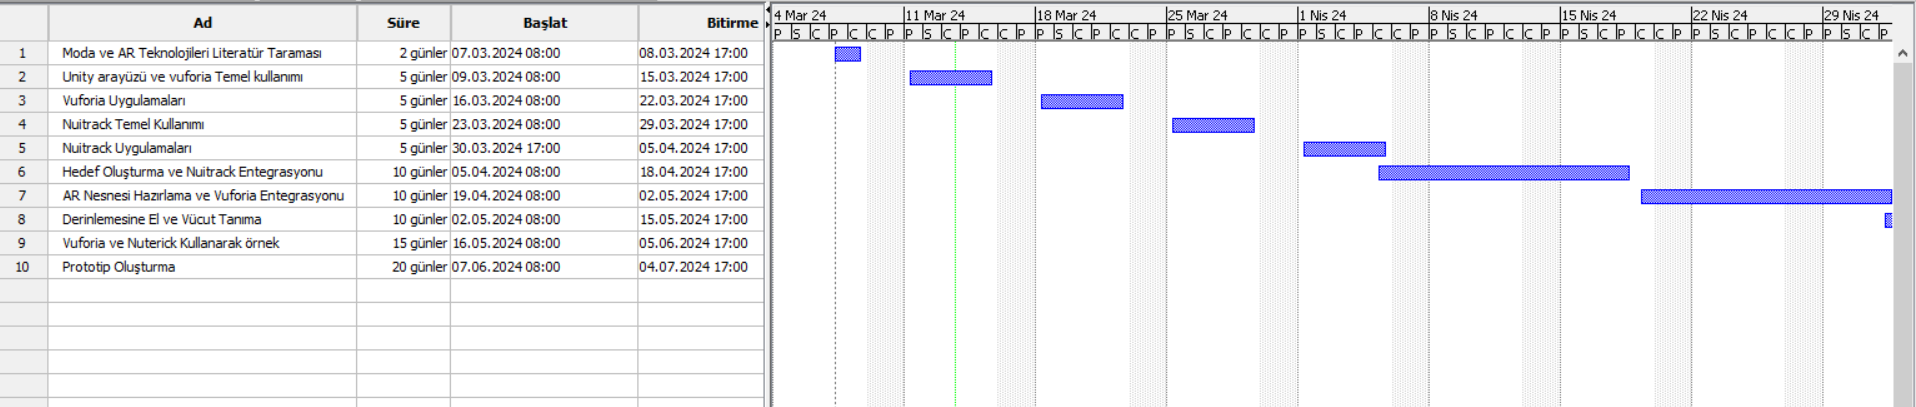
\includegraphics[angle=0, width=\textwidth]{Ekran.png}
    	
    	\label{gantt}
    \end{figure}
	%Kaynakçayı yazdırmak
	\bibliographystyle{ieeetr}
	\bibliography{references.bib} 
	%\printbibliography %Prints bibliography
	
	
	
\end{document}